\CourseSection{Testing and Evaluation}\label{sec:testing}

\Guidance{Describe how the team expects to test the proposed system. The purpose
of this section is to show that testing has been considered, not to provide a
complete test procedure. (This you will do in the blueprint.) Use a diagram to communicate the overall test approach
and briefly explain the expected evidence of success.}

\begin{figure}[!htb]
\centering
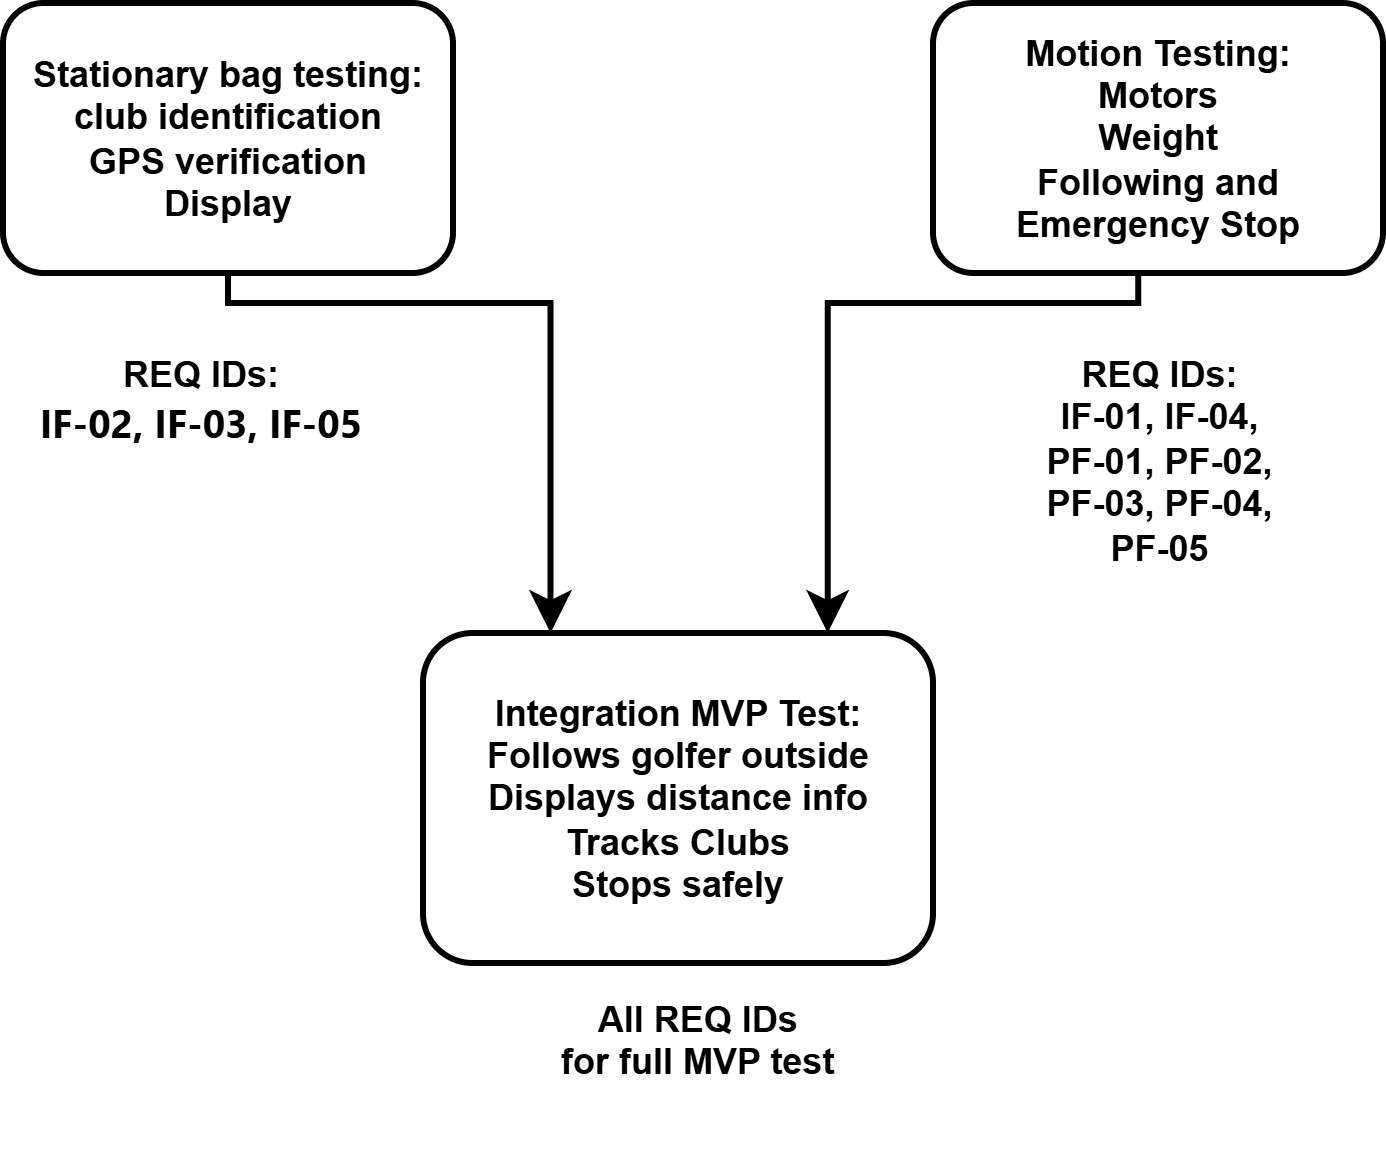
\includegraphics[width=0.5\linewidth]{figures/testing-and-evaluation.png}
\caption{Proposed testing approach: stationary bag testing and motion testing are completed separately, with their requirement IDs, before the integrated MVP test.}
\label{fig:test-approach}
\end{figure}

Testing is staged: each subsystem is tested on its own first, and the cart is tested as a whole once all of them work. Table~\ref{tab:test-plan} links each stage to the specification IDs in Table~\ref{tab:proposal-specs}, and Table~\ref{tab:test-plan-full} in Appendix~\ref{app:test-plan} gives the procedure and expected evidence of success for each. These tests verify the requirements, and they need only a controlled grass area, a tape measure, a laser rangefinder for reference distances, and video for timing. Validation is a final trial in which a golfer plays a hole using only the cart, with no phone. A safety operator holding the emergency stop is present for every test in which the cart moves.

\begin{TableBlock}
\small
\captionof{table}{Summary of the proposed test stages and the specifications each one verifies.}\label{tab:test-plan}
\begin{tabularx}{\linewidth}{@{}YYYY@{}}
\rowcolor{MidGray}
\TableHeader{Mobility and safety} & \TableHeader{Club identification} & \TableHeader{GPS and display} & \TableHeader{Range} \\
\midrule
IF-01, IF-04, PF-01, PF-02, PF-03, PF-05 & IF-03 & IF-02, IF-05 & PF-04 \\
\addlinespace[3pt]
Following, obstacle, and emergency-stop trials on grass & Club removal and return with the bag stationary & Displayed distance against reference distances & Loaded run on one charge \\
\bottomrule
\end{tabularx}
\end{TableBlock}

\Guidance{List as many verification and validation tests as you can think of at this time. Briefly identify any equipment, software, facilities, or special
conditions expected to be needed. Explain how the tests will help
determine whether the final system meets its main requirements (verification) and stakeholder
needs (validation).}
